\section{DGFE Theory}

We begin with equation \ref{g_mu_treq}; the within group $g$, within angle $n$ 1D transport equation.  In the following section we drop the group subscript and angle superscript and set $Q(x)=0$.

\begin{equation}
\mu \frac{\partial}{\partial x} \psi(x) + \Sigma_t \psi(x) = S(x)
\label{1d_tr_dg}
\end{equation}
Equation \ref{1d_tr_dg} is a first order, linear, hyperbolic ordinary differential equation, as such the methods introduced in chapter 6
(even parity transport) of E. E. Lewis’s computational methods in radiation transport largely do not apply. The even parity formulation of the transport equation contains a spatial derivative of order 2 results
in certain nice aspects to the DGFE discretized equations – primarily that even order equations yield
symmetric matrices after discretization. The even parity formulation of the transport equation is not pursued here
since it has difficulty including anisotropic scatter \cite{Lewis}. It is possible to use the Petrov-Galerkin method
on the first order equation without constructing the second order form of the transport equation.

First, we multiply both sides of equation \ref{1d_tr_dg} by a yet to be defined test function, $v(x)$ resulting in:
\begin{equation}
\mu \frac{\partial}{\partial x} \psi(x) v(x) + \Sigma_t \psi(x)v(x) = S(x)v(x)
\label{1d_tr_dg2}
\end{equation}
Next the equation is integrated over the domain, $x \in [0, L]$:
\begin{equation}
\int_0^L \mu \frac{\partial \psi(x)}{\partial x} v(x) dx + \int_0^L \Sigma_t \psi(x)v(x) dx =  \int_0^L S(x)v(x) dx
\label{1d_tr_weak}
\end{equation}
This is known as the weak form of equation \ref{1d_tr_dg}.
See Appendix A for background on the weak form of the equation.

Next, we integrate the first term in \ref{1d_tr_weak} by parts giving:
\begin{equation}
\mu \psi(x)v(x)|_0^L- \mu \int_0^L  \psi(x) \frac{\partial v(x)}{\partial x} dx + \int_0^L \Sigma_t \psi(x)v(x) dx =  \int_0^L S(x)v(x) dx
\label{1d_tr_weak2}
\end{equation}
We are free to choose a functional form for $v(x)$. In the Galerkin approach, the test function is
taken to be of the same functional form as the solution approximation $\psi(x)$. The simple DGFE choice is to take $v(x)$ to be a
linear combination of ramp functions. Each ramp function $h_{ei}(x)$ is supported only at one nodal location in the mesh
and is defined to be zero at all other nodes. Figure \ref{single_ele} displays two interior neighboring ramp functions which are each non-zero over element $e_1$. The ramp functions are defined to have unit height over their supporting node.  An element is defined to be the region between bounding nodes which are points at which the solution is supported.  For simplicity all elements are assumed to have width $\Delta x$.

\begin{figure}[!htbp]
\centering
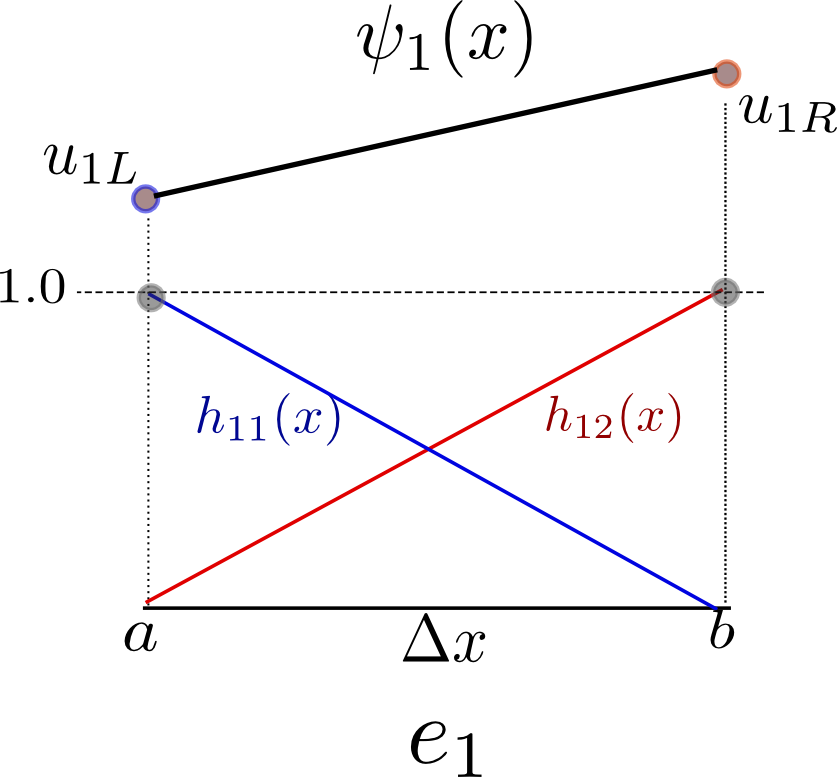
\includegraphics[width=5cm]{images/single_ele.png}
\caption{Single finite element.}
\label{single_ele}
\end{figure}

\begin{figure}[!htbp]
\centering
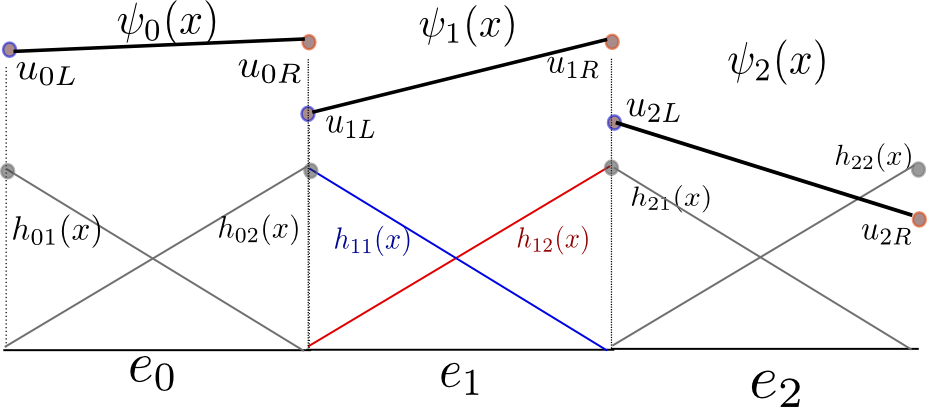
\includegraphics[width=8cm]{images/multi_ele.png}
\caption{Multiple DG finite elements.}
\label{multi_ele}
\end{figure}

In practice the transport equation is integrated element-by-element, rather than over the whole domain.  The contribution of each element will be summed together to recover the neutron balance over the whole domain.  For now, we consider an interior element, $e_1$ defined on the sub-region: $[a, b]$.  Figure \ref{multi_ele} shows the interior element $e_1$ bounded by two other elements.  Note that the hypothetical DGFE numerical solution $\psi$ jumps in value at element boundaries.  As a consequence, at element boundaries the solution is double value (in 1D, in higher dimensions it could be $N$-valued).  This is where the Discontinuous Galerkin finite element scheme differs from the more commonly known Continuous Galerkin (CG) FE spatial discretization method.

Now it is useful to formally define the ramp functions and their linear combination.  Over a single element, the solution $\psi_e(x)$ is given by equation \ref{sol_ele}.

\begin{equation}
\psi_e(x) = u_{eL}h_{e1}(x) + u_{eR}h_{e2}(x) = \sum_i u_{ei} h_{ei}(x),\ x\in[a,b]
\label{sol_ele}
\end{equation}
Where $i$ is the edge index, in the one dimension case this denotes either the left or right face.
The ramp functions are given as:
\begin{equation}
  h_{e1}(x) =
  \begin{cases}
                                   \frac{-1}{\Delta x}(x-a) + 1 & \text{, $x\in[a,b]$} \\
                                   0 & \text{, $otherwise$} 
  \end{cases}
\end{equation}
and
\begin{equation}
  h_{e2}(x) =
  \begin{cases}
                                   \frac{1}{\Delta x}(x-a) & \text{, $x\in[a,b]$} \\
                                   0 & \text{, $otherwise$} 
  \end{cases}
\end{equation}
As previously stated, the Galerkin approach is to enforce \ref{gal_asm}.
\begin{equation}
\psi_e(x) = v_e(x)
\label{gal_asm}
\end{equation}
on each element.  At first glance this appears this is an arbitrary choice, and indeed, this assumption does not have to be made.  One could use different functional families for $\psi$ and $v$, however we will not investigate this option.

For this case where we have chosen simple ramp functions to represent our 1D solution approximation, each element has two unknown scalar values, $\{u_{eL}, u_{eR}\}$ that act to scale the ramp functions over the element.

\begin{equation}
\mu \psi_e(x)v_e(x)|_a^b- \mu \int_a^b  \psi_e(x) \frac{\partial v_e(x)}{\partial x} dx + \int_a^b \Sigma_t \psi_e(x)v_e(x) dx =  \int_a^b S_e(x)v_e(x) dx
\label{1d_tr_weak_ele}
\end{equation}

Next we apply \ref{sol_ele} and \ref{gal_asm} to \ref{1d_tr_weak_ele}.
The solution over the entire domain is the summation of the piecewise linear solution approximation over all elements:
\begin{equation}
\psi(x) = \sum_{e=0}^M \psi_e(x) 
\end{equation} 
Where $M$ is the number of finite elements used.
 
The integral terms in equation \ref{1d_tr_weak_ele} can be expanded to explicitly show their dependence on the scaling factors.  The second term in \ref{1d_tr_weak_ele} integrates to \ref{w_e}.

\begin{equation}
W_e = -\int_a^b \mu \psi_e \frac{\partial v_e}{\partial x} dx = \frac{-1}{2\mu}(u_{eR}^2 - u_{eL}^2) = 
\frac{-1}{2\mu} \mathbf u_e 
\begin{bmatrix}
    -1      & 1 \\
    -1       & 1 
\end{bmatrix}
\mathbf u_e^T
\label{w_e}
\end{equation}
With $\mathbf u_e = [u_{eL}, u_{eR}]$.  Note that this produces an asymmetric element matrix.  As a consequence, it is required that the order of the nodes from left to right is preserved.

The third term in \ref{1d_tr_weak_ele} integrates to \ref{m_e}.
\begin{equation}
M_e = \int_a^b \Sigma_t \psi_e(x)v_e(x) dx =
\frac{\Sigma_t \Delta x}{3} (u_L^2 + u_L u_R + u_R^2) = 
\frac{\Sigma_t \Delta x}{3} \mathbf u_e 
\begin{bmatrix}
    1      & 1/2 \\
    1/2      & 1 
\end{bmatrix}
\mathbf u_e^T
\label{m_e}
\end{equation}

The RHS of equation \ref{1d_tr_weak_ele} integrates to \ref{s_e}.

\begin{equation}
RHS_e = \int_a^b S_e(x)v_e(x) dx =
\frac{S_e \Delta x}{2} (u_L + u_R) = 
\frac{S_e \Delta x}{2}
\begin{bmatrix}
    1     \\
    1 
\end{bmatrix}
\mathbf u_e^T
\label{s_e}
\end{equation}

Where we take the value $S_e$ to be the value of $S_e(x)$ at the element mid-point.  This is valid provided that $S_e(x)$ is a linear function since this is equal to the average value of $S_e(x)$ over the element.

Finally, we must deal with the boundary term which arose from integrating the first term of equation \ref{1d_tr_weak_ele} by parts.  This term is the only term which will contain information from neighboring elements in its definition.  This is why it is said that the DGFE technique is ``compact''. Let the outward normal at a given element boundary to be denoted by $\mathbf n$.  The left side outward normal for element $e_1$ is depicted in figure \ref{bound_norm}.

\begin{figure}[!htbp]
\centering
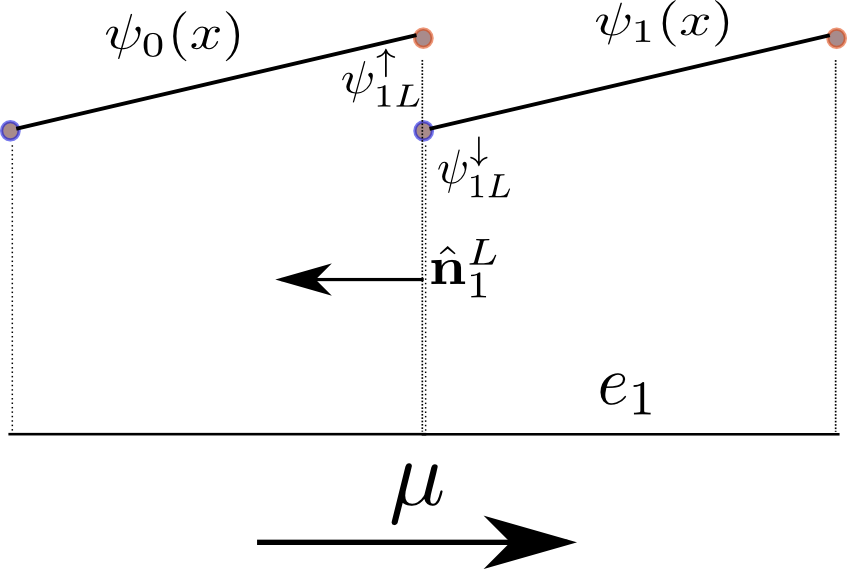
\includegraphics[width=8cm]{images/bound_norm.png}
\caption{Outward normal on left face of element $e_1$. As drawn, $\psi_{1L}^{\uparrow}=u_{e_0, 2}$ and $\psi_{1L}^{\downarrow}=u_{e_1, 1}$ in the figure.}
\label{bound_norm}
\end{figure}

It is useful to define a jump and average condition on an element boundary.
The average condition at the junction between two elements is given by \ref{avg}.
\begin{equation}
\{\{u\}\}_p = \frac{1}{2} (\lim_{x \to p^+} u_{p} + \lim_{x \to p^-} u_{p})
\label{avg}
\end{equation}
Where the subscript $p$ denotes evaluation at a boundary. Since $\psi(x)|_p$ and therefore $u_p$ is double valued at the element boundaries; the limit approaching from the left is not equal to the limit approaching from the right.

And the jump is provided by equation \ref{jmp}.
\begin{equation}
[[u]]_p =  (\lim_{x \to p^+} u_{p} - \lim_{x \to p^-} u_{p})
\label{jmp}
\end{equation}

Now it is useful define the ``upwind'' flux.  According to \ref{upwind}, the sign of the dot product between the current neutron flow direction, $\mu$ and the boundary normal vector $\mathbf n_{e,p}$ can be used at each edge to determine the upwind flux value.

\begin{equation}
\psi^{\uparrow} = 
  \begin{cases}
      \psi_k|_p & \text{if $\mu \cdot \mathbf n_e|_p \leq 0$} \\
      \psi_e|_p & \text{if $\mu \cdot \mathbf n_e|_p > 0$} 
  \end{cases}
\label{upwind}
\end{equation}
Where $k$ represent the neighboring element and $e$ is the current element.

It is unclear what value to choose for the flux at the element boundaries.  This is required to evaluate $\mu \psi_e(x) v_e(x)|_a^b$ in \ref{1d_tr_weak_ele}. The DGFE method introduces the numerical flux $\mu \cdot \mathbf n \hat{F} $ to resolve this issue.  The boundary term becomes \ref{dg_fe_bound}.

\begin{equation}
\mu \psi_e(x) v_e(x)|_a^b = \mu \cdot \mathbf n \hat{F}  v_e(x)|_a^b 
\label{dg_fe_bound}
\end{equation}

\subsubsection{Upwind Formulation}
In this case, when evaluating $\mu \psi_e(x) v(x)|_a^b$, $\psi(x)$ always takes the upwind value at element boundaries.

\begin{equation}
\mu \cdot \mathbf n \hat{F}  = \mu \cdot \mathbf n \psi^{\uparrow} 
\end{equation}

This makes physical sense if the neutrons are constrained to flow in the direction $\mu$ by the discrete ordinates approximation.  The value of angular dependent neutron flux at the element boundaries should depend only on the neutron's behavior immediately upstream of the boundary.  In other words, all neutron interactions downstream of the boundary do not have a large influence on the upstream flux.  This is true particularly in the case of the once-scattered flux.  It was not discussed in this work, but equation \ref{1d_tr_weak} is written for a single scattering source iteration (SI), which means equation \ref{1d_tr_weak} is equivalent to the one-scattered transport balance.  For more information on source iteration, see E.E. Lewis's text \cite{Lewis}.

Equation \ref{dg_fe_bound} can now be evaluated.
If $\mu \cdot \mathbf n \leq 0$: 
\begin{equation}
B_{ep_1} = \mu \cdot \hat{\mathbf n} \hat{F}  v(x)|_{p_1} = 
\mu \cdot \mathbf n (u_e^2)|_p = 
(\mu \cdot \mathbf n) \mathbf u_p 
\begin{bmatrix}
    1      & 0 \\
    0      & 0 
\end{bmatrix}
\mathbf u_p^T
\end{equation}
Where $\mathbf u_p = [u_e, u_k]|_p$.  Again, $u_k|_p$ is the value of $\psi$ as the neighboring element approaches the boundary (i.e $u_k=\lim_{x \to p^k}\psi(x)$)  and likewise, $u_e|_p=\lim_{x \to p^e}\psi(x)$.

If $\mu \cdot \mathbf n > 0$:
\begin{equation}
B_{ep_2} = \mu \cdot \hat{\mathbf n} \hat{F}  v(x)|_{p_2} = 
\mu \cdot \mathbf n (u_e \cdot u_k)|_p = 
(\mu \cdot \mathbf n) \mathbf u_p 
\begin{bmatrix}
    0      & 0 \\
    1      & 0 
\end{bmatrix}
\mathbf u_p^T
\end{equation}

And the sum over both edges is given by \ref{ele_sum}.
\begin{equation}
 B_{ep_1} + B_{ep_2} = \mu \cdot \hat{\mathbf n} \hat{F}  v(x)|_a^b
\label{ele_sum}
\end{equation}

\subsubsection{Average Flux Formulation}
Alternatively, instead of simply taking the upwind flux value at each element boundary, one may choose to use the average flux at each boundary.  This results in the following:

If $\mu \cdot \mathbf n \leq 0$: 
\begin{equation}
B_{ep_1} = \mu \cdot \hat{\mathbf n} \hat{F}  v(x)|_{p_1} = 
\mu \cdot \mathbf n 0.5 (u_e + u_k)|_p = 
(\mu \cdot \mathbf n) \mathbf u_p 
\begin{bmatrix}
    0.5     & 0 \\
    0.5     & 0 
\end{bmatrix}
\mathbf u_p^T
\end{equation}
and
If $\mu \cdot \mathbf n > 0$:
\begin{equation}
B_{ep_2} = \mu \cdot \hat{\mathbf n} \hat{F}  v(x)|_{p_2} = 
\mu \cdot \mathbf n 0.5 (u_e + u_k)|_p = 
(\mu \cdot \mathbf n) \mathbf u_p 
\begin{bmatrix}
    0.5     & 0 \\
    0.5     & 0 
\end{bmatrix}
\mathbf u_p^T
\end{equation}

This formulation makes physical sense in the case that upstream and downstream interactions influence the value of the flux at element boundaries.  In the purely diffusive case, where Fick's law holds, this assumption is valid an therefore the average flux is a good choice.  In the case of the hyperbolic first order equation \ref{1d_tr_weak}, the average boundary flux formulation might lead to unphysical results.

\subsubsection{System Matrix Construction and Boundary Conditions}

The goal is to find the combination of the scaling factors on all elements simultaneously which best satisfies the overall weak form of the neutron balance equation \ref{1d_tr_weak}.  One can think of the finite element method in an optimization context in which some (hopefully unique) combination of the scalars $\{u_0, u_1, ...\}$ reduces the residual of \ref{1d_tr_weak} to some minimal value.
 
 To construct the system matrix A, the individual element matrices are ``stamped'' into A. Since
each node is assigned a unique ID the elements of A e can be copied into the global A.
 
Up until this point we have disregarded the application of boundary conditions since we focused on the interior elements.  For the first order transport equation, all boundary conditions (vacuum, reflective, white) can be
described as either fixed or free. A Fixed boundary condition specifies the value of $\psi$ at the boundary.
This arises in the vacuum case where inward facing ordinate fluxes are set equal to zero at the
boundary. This also arises in the reflective and white cases where the banked outward fluxes from the
previous scattering source iteration are assigned as fixed boundary values for the inward facing ordinate
fluxes. A free boundary arises in cases where the flux is allowed to escape from the domain.
To implement a fixed boundary condition, the row in the global system matrix, A, corresponding
to the boundary node is set equal to zero at all elements except at the diagonal where the diagonal
entry is set equal to 1. On the right hand side the specified value for the flux at that node is set.
Free boundary conditions require no action.